\section{GOAL}
We have implemented GAMYGDALA as a plugin in the existing GOAL source code. To do this, we first need to have a good overview of the GOAL architecture.

\subsection{GOAL architecture overview}
The GOAL source consists of two major parts: the grammar and the runtime. These parts can be characterised as the parser and interpreter respectively. In both these parts we have had to hook in our plugin. We will discuss the relevant parts of both the grammar architecture and the runtime architecture, and how we embedded our custom actions in these architectures.

\subsubsection{Grammar overview} 
The grammar uses the antlr4 library to create clear grammar in .g4 files. It then uses this grammar to parse the program. We need to make sure that our custom action (also referred to as plugin) is correctly inserted in the existing grammar. \\ 

The parsing consists of multiple levels. The first level is converting the plain text to collections of very basic expressions. The second level turns these basic expressions into clearer expressions. In this level, every action has its own class, for example. We needed to make sure that such an action exists for each of our custom actions, and that it is created when necessary. \\

All of our custom actions share the same format, that is to say they all take a list of values as their parameters instead of some predicate. Since these actions all share this format, it makes sense to generalise them. This is exactly what we have done. There is an abstract 'parameter action', and to create a new action in the grammar we only need to create a new class for it in a certain package. 

The classes that handle the second level of parsing are called validators, because they not only parse the program but also make sure that everything is correct. The grammar has four different validators for the four parts of the goal language: agents, multi-agent systems, modules and tests. Most relevant for us are the agents; we need to make sure that our custom action passes the validation of the agent's execution code, and also that the parameters that are passed to the action are preserved in the process. \\ 

To make sure that this agent validator class did not become much larger than it already was, we created a parameter action factory that handles the creation of the parameter actions. Using a class loader, this factory creates the specific parameter action that matches the operator. This is very easy, because every parameter action executor has an 'Action Token' annotation that tells the class loader for which operator it is used. To allow for easy class loading, the reflections package was used.

The grammar is not responsible for any communication with the actual implementation of the plugin; it just makes sure that an action is created, and the parameters, though not yet interpreted, are passed to it.

\subsubsection{Runtime overview}
In this section, the parts of the runtime that are relevant to the implementation of our custom action will be covered. In the runtime changes were made to allow for interpretation of the custom actions, and the actual interpretation is hooked to the interface between GOAL and GAMYGDALA. \\ 

The runtime traverses the rules of the agent program, and when it crosses an action, it creates an action executor for said action. This action executor is then executed. We needed to make sure that such an action executor exists for each of our custom actions. \\

Since all actions still share the same format, generalisation could also be applied  in the runtime. We created an abstract 'parameter action executor', which all specific action executor implementations extended. Each action executor specifies for which action it is an executor.

All these action executors are put together in the same package. That way, the runtime can easily find the action executor that matches that action is has come across. Again, a factory that uses the reflections package was used, although this time annotations were not necessary. In this case, we could simply use type parameters, since we were now trying to match an action type instead of an operator integer. This way, the code also became cleaner, because by using type parameters a parameter action executor could never be used for the wrong type of parameter action.

Once the action executor is found and actually executes, the call is forwarded towards the GOAL-GAMYGDALA. Since this interface is built so that GOAL does not have to know anything at all about GAMYGDALA except for the actions it provides, the raw GOAL terms are passed to the interface.

In some cases, the emotions of the agent need to be updated after execution. For this purpose, we have created an emotion manager class. This class is responsible for updating the emotions in the mental state of the agent.

\subsection{Design Patterns}
Several design patterns were used in the code we added to GOAL. This section provides an overview of those design patterns.

\subsubsection{Factory Method pattern}
In both the grammar and the runtime, we needed a way to create actions and action executors, based on operators and actions respectively. To make sure that this responsibility was separated from the rest of the GOAL source, we decided to create a factory in both cases. To make sure we also adhered to the open/closed principle, we decided to expand this to the Factory Method Pattern. By using this specific pattern, a new factory can always be created and substituted for the old factory in case anyone wants to implement a new way to create these actions and action executors. This pattern and its use are clearly visible in the UMLs of both the grammar and the runtime.

\subsubsection{Strategy pattern}
In the runtime, there was already a strategy pattern in place for the actions, but as you might have noticed, we decided to take one step further and also implement the strategy pattern for the so-called parameter action executors. They are, in essence, all interchangeable, since they all 'execute something'. It is up to the factory to determine which of these executors is appropriate for the current action.

\subsubsection{Singleton pattern}
For the emotion manager, we have used the Singleton pattern. This allowed us to encapsulate the emotion updating functionality in a new class, while not having to instantiate this class countless times, wasting a lot of memory.

\begin{figure}
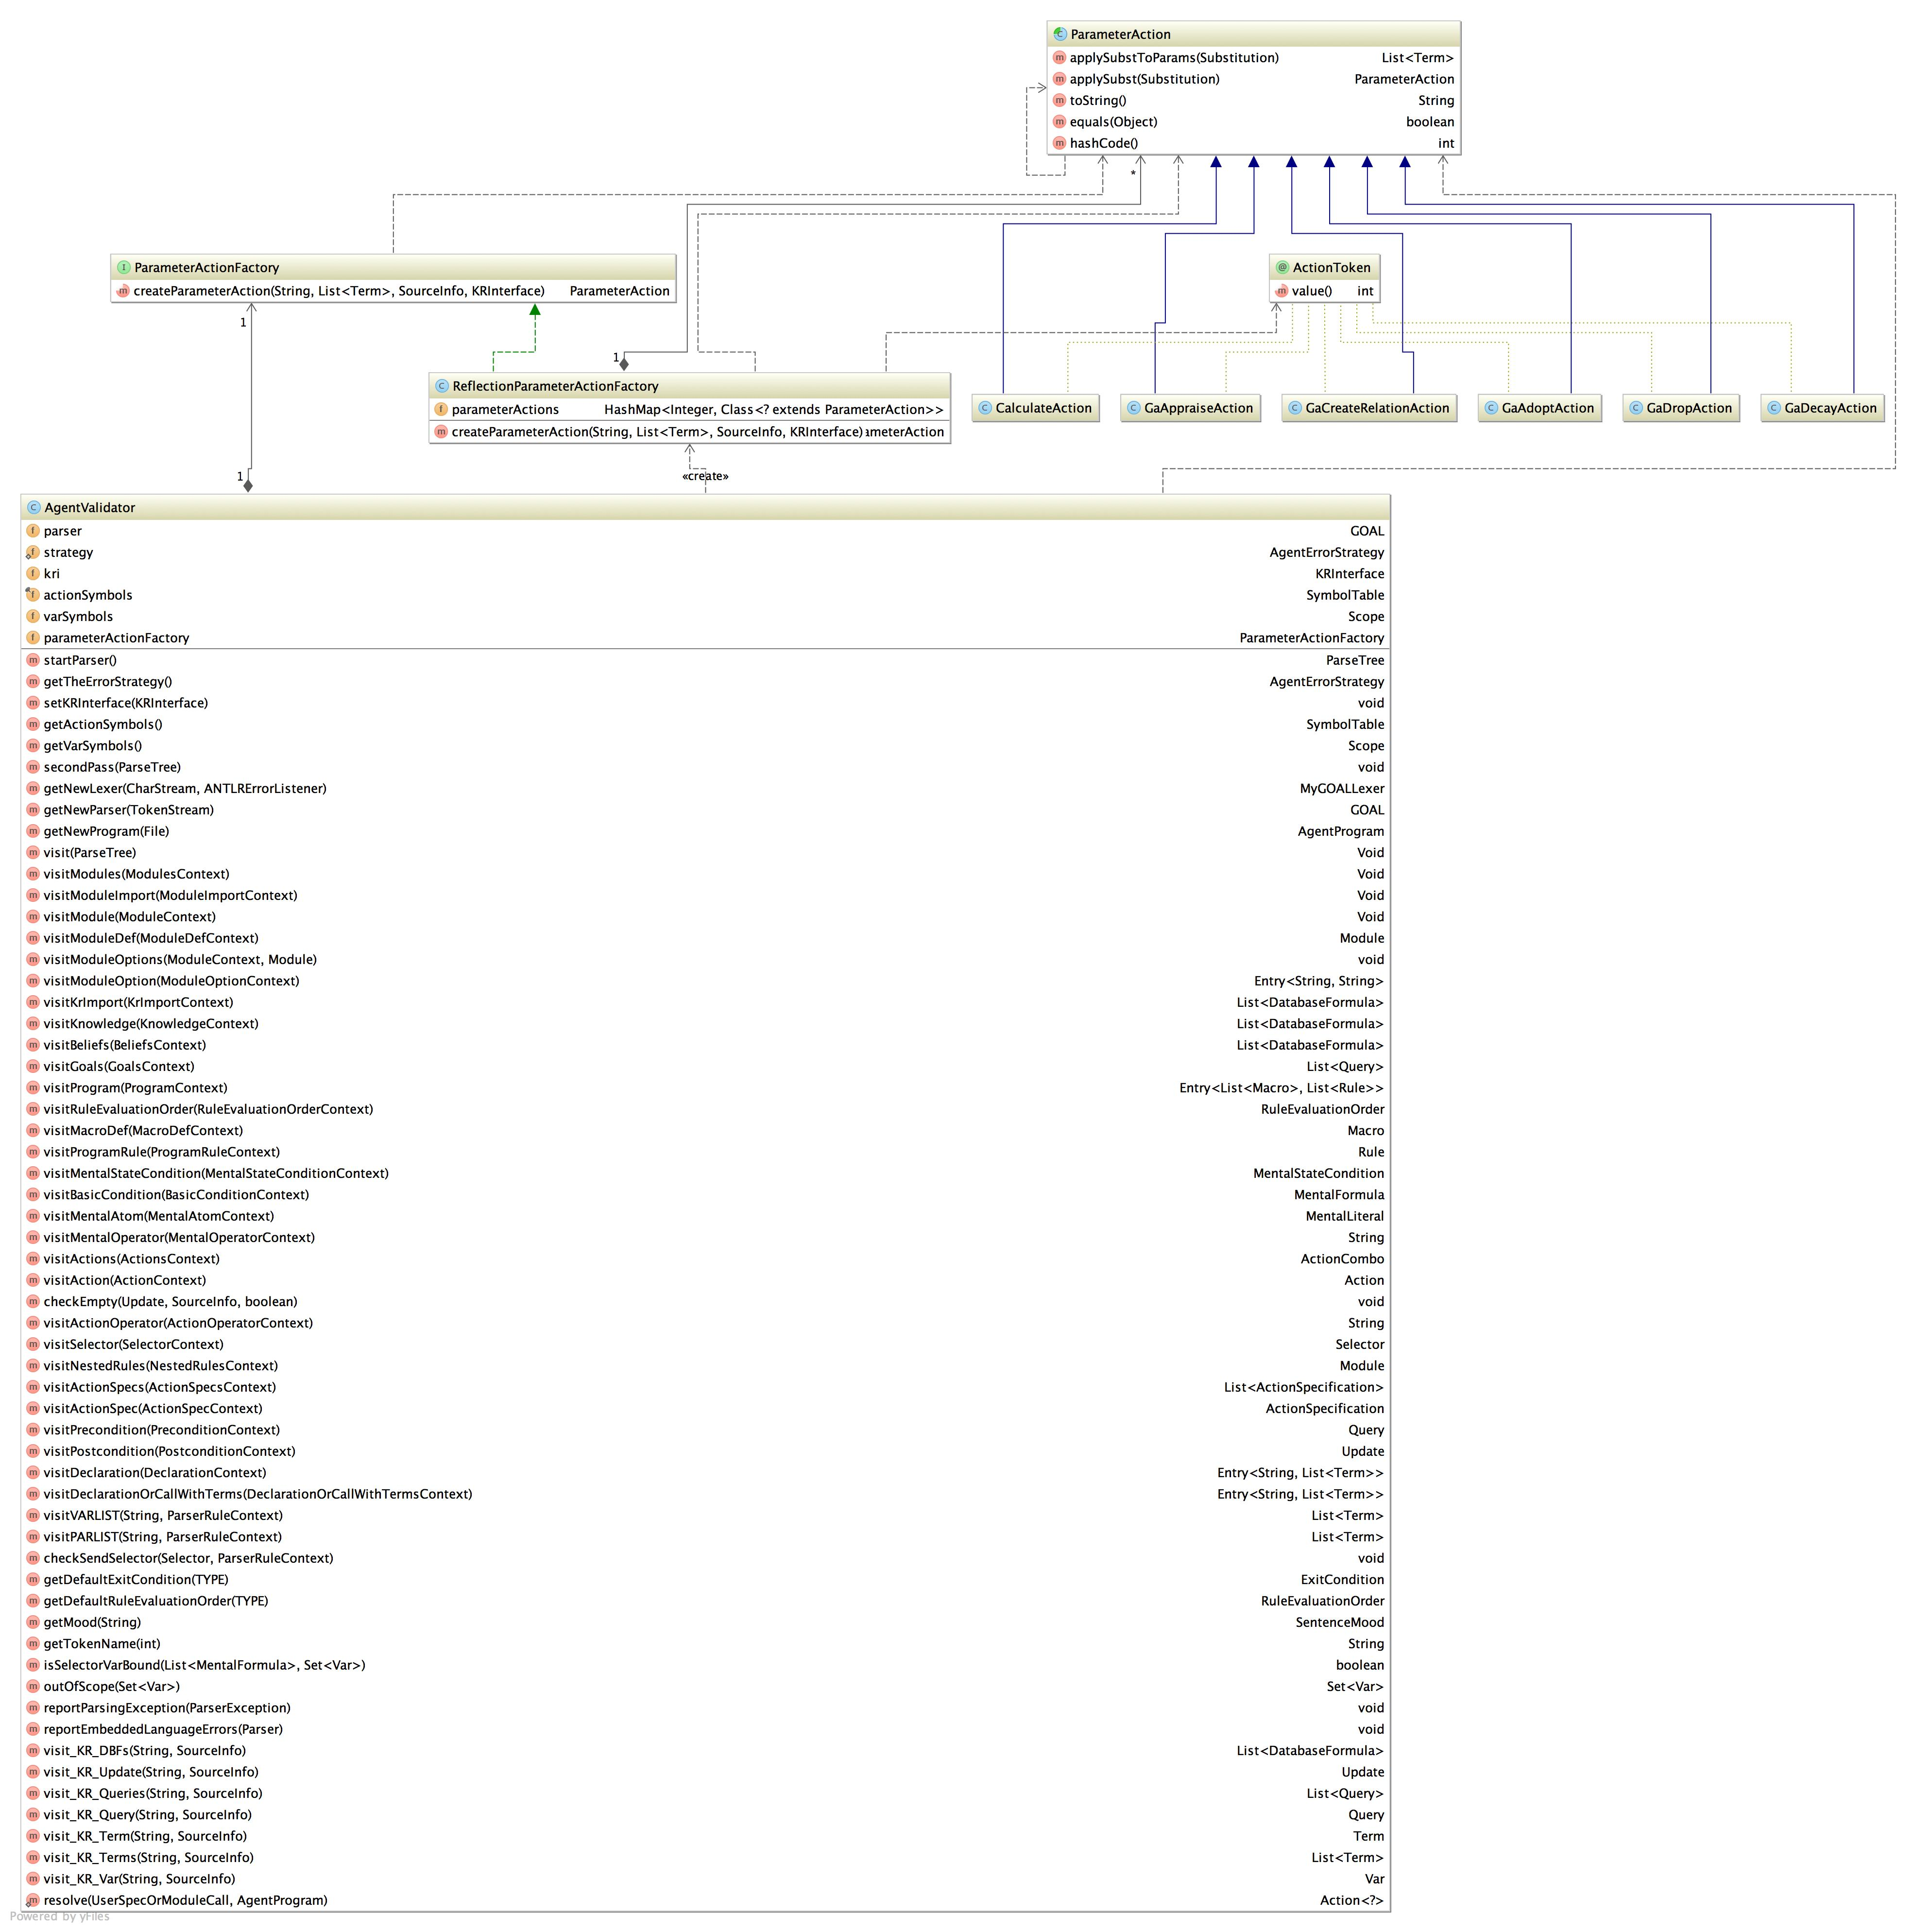
\includegraphics[width=\linewidth]{diagram-grammar}
\caption{The UML-diagram for the grammar.}
\end{figure}

\begin{figure}
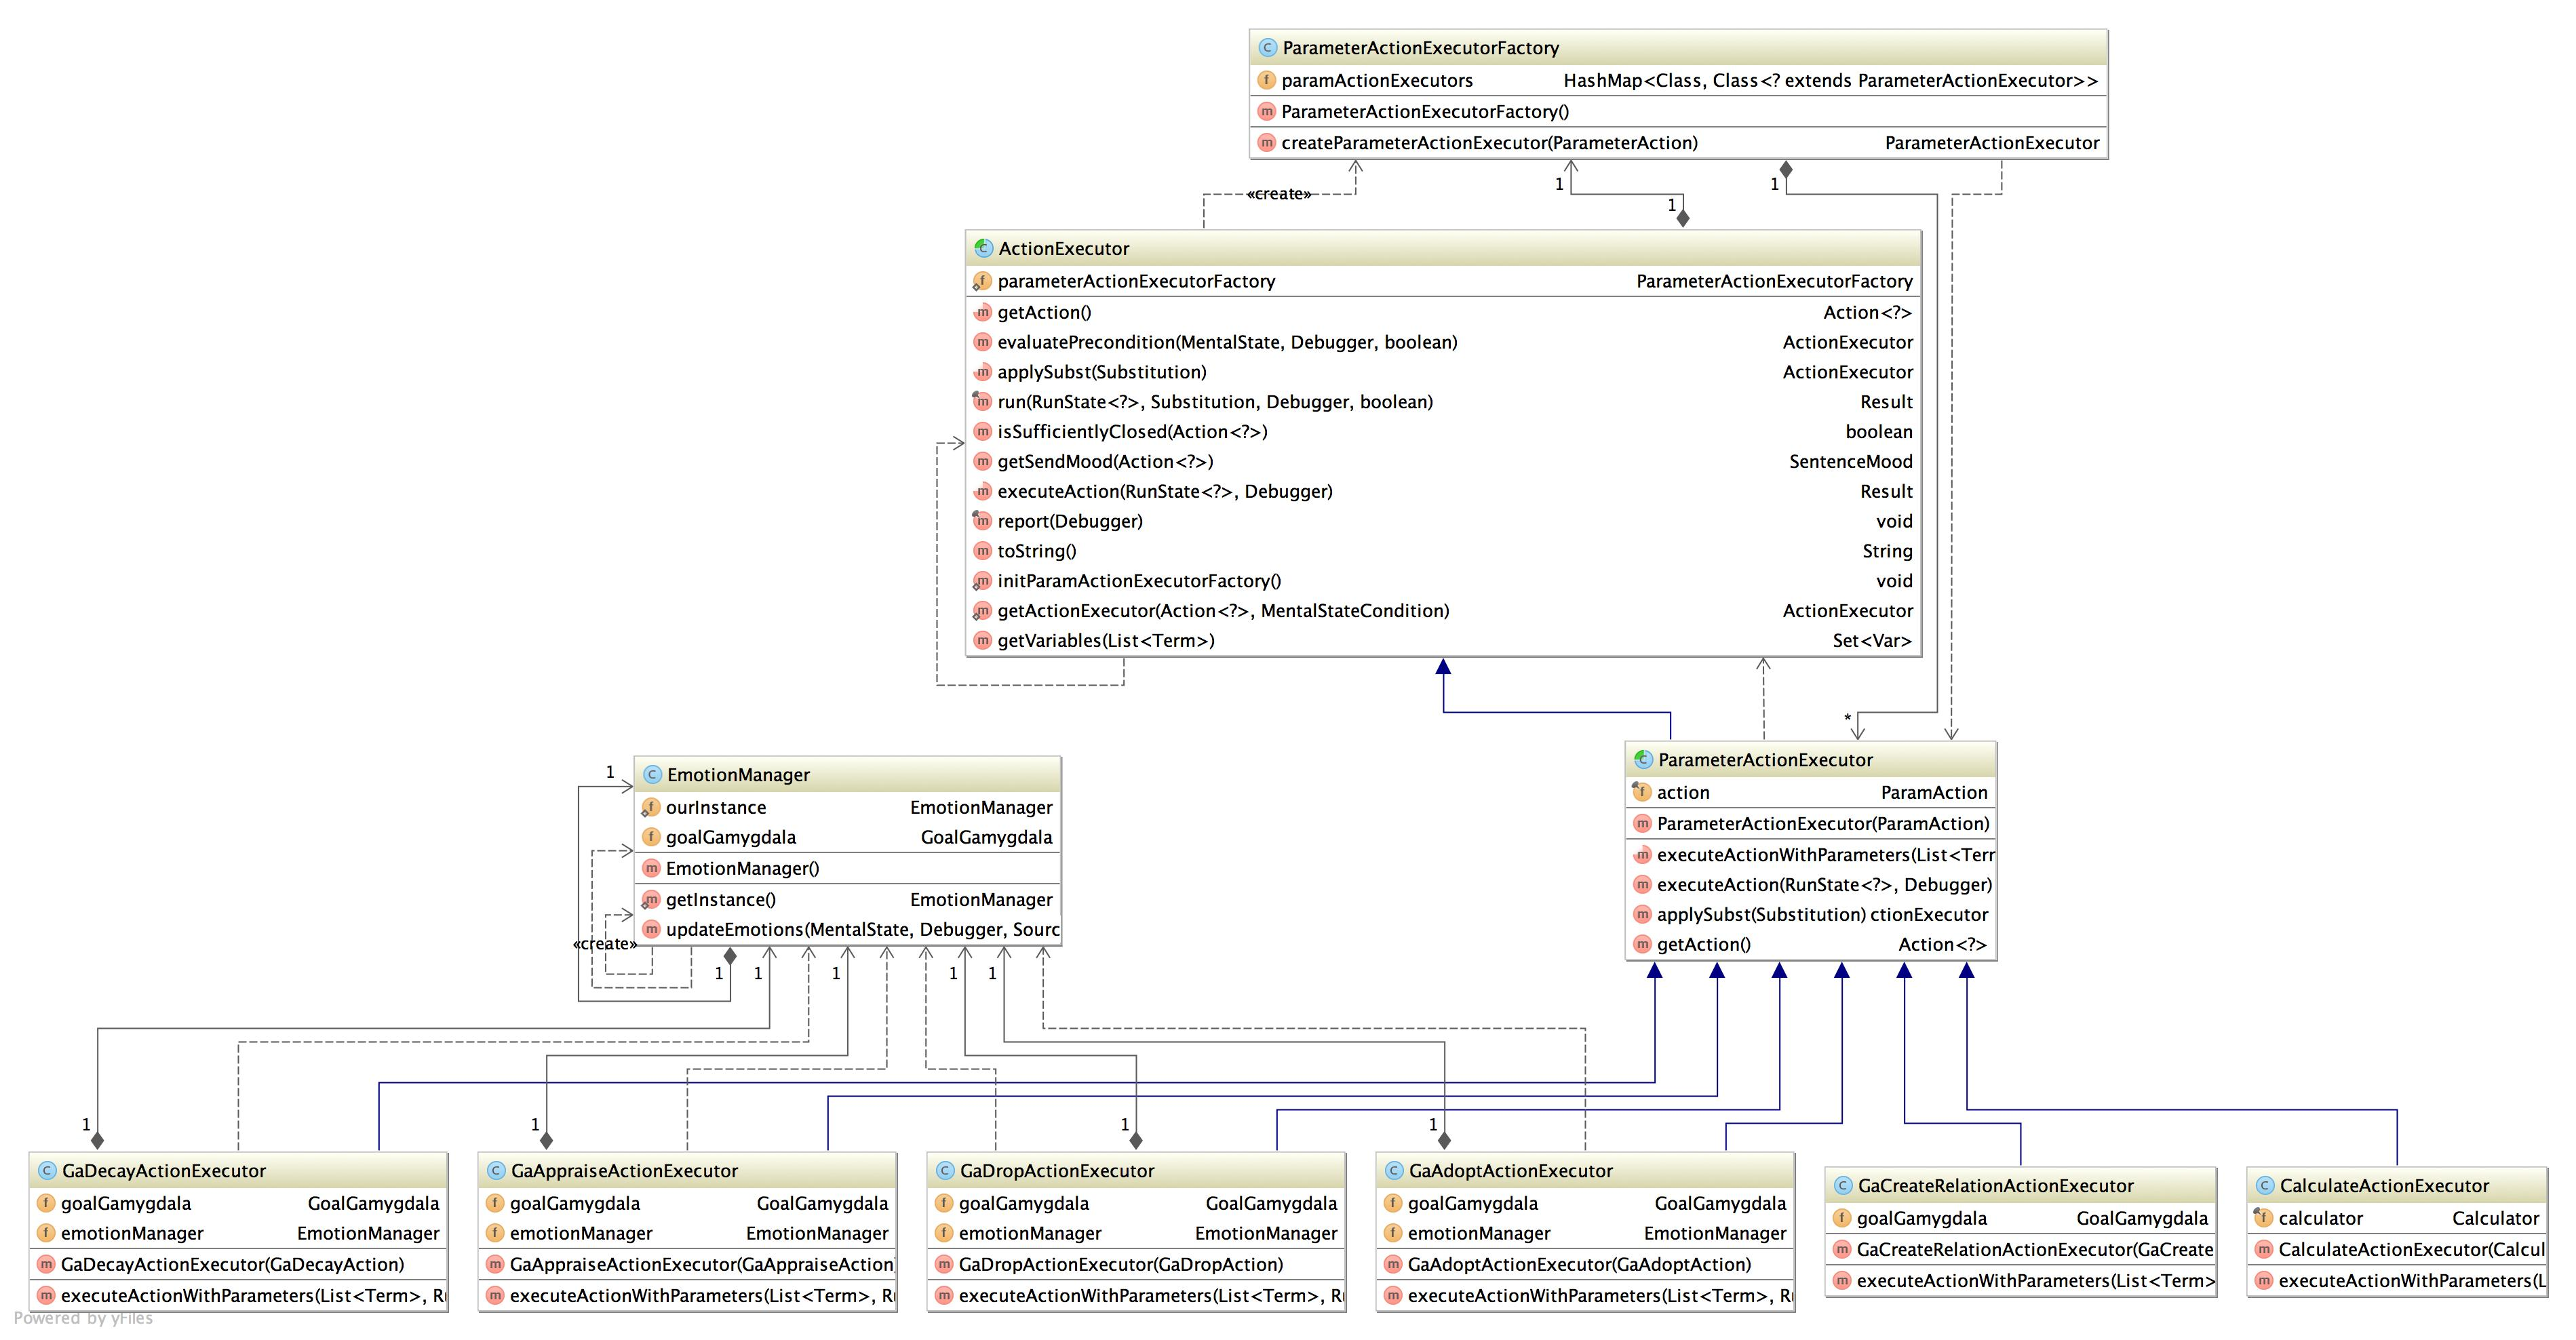
\includegraphics[width=\linewidth]{diagram-runtime}
\caption{The UML-diagram for the runtime.}
\end{figure}